\documentclass[xcolor={table}]{beamer}
\usepackage{pgfgantt}
\usepackage[utf8]{inputenc}
\usepackage{cite}

% Math
\usepackage{amsmath}
\DeclareMathOperator\erfc{erfc}
\usepackage{nicefrac}
% For tables
\usepackage{tabularx, booktabs}
\usepackage{multirow}

% Units
\usepackage{siunitx}
\sisetup{
    exponent-product = \cdot,
    separate-uncertainty = true,
    per-mode = symbol,
    group-digits = false,
    detect-weight=true,
    detect-family=true,
    detect-all
}
\DeclareSIUnit{\sqrthz}{\ensuremath{\sqrt{\text{\hertz}}}}
\DeclareSIUnit{\voltnoise}{\volt\per\sqrthz}
% Tikz
\usepackage[europeanresistors,americaninductors, americancurrents, american voltages, siunitx]{circuitikz}
\usepackage{tikz}
\usetikzlibrary{shapes,arrows, calc, automata, positioning, chains, decorations.markings, calc, patterns, angles, quotes}
\usepackage{pgfplots}
\pgfplotsset{compat=1.16}

\usepackage{graphicx} % Figures/graphics
\usepackage{float} % Floats, H
% Subfigures:
\usepackage[caption=false, font=normalsize, labelfont=sf, textfont=sf]{subfig}

\title{Specialization Project - Weekly meeting}
\author{Fredrik Feyling}
\date{\today}

\begin{document}

\frame{\titlepage}

% ------------------- Since last week ---------------- %
\begin{frame}
\frametitle{Since last week}
\begin{columns}

\column{0.5\textwidth}
\begin{itemize}
\item Started writing script for simulating ADC and LNA
\item Written classes for ADC, LNA and Signal Generator
\item Function for analysing SNR and plotting PSD
\end{itemize}

\column{0.5\textwidth}
\begin{figure}[htbp]
\begin{center}
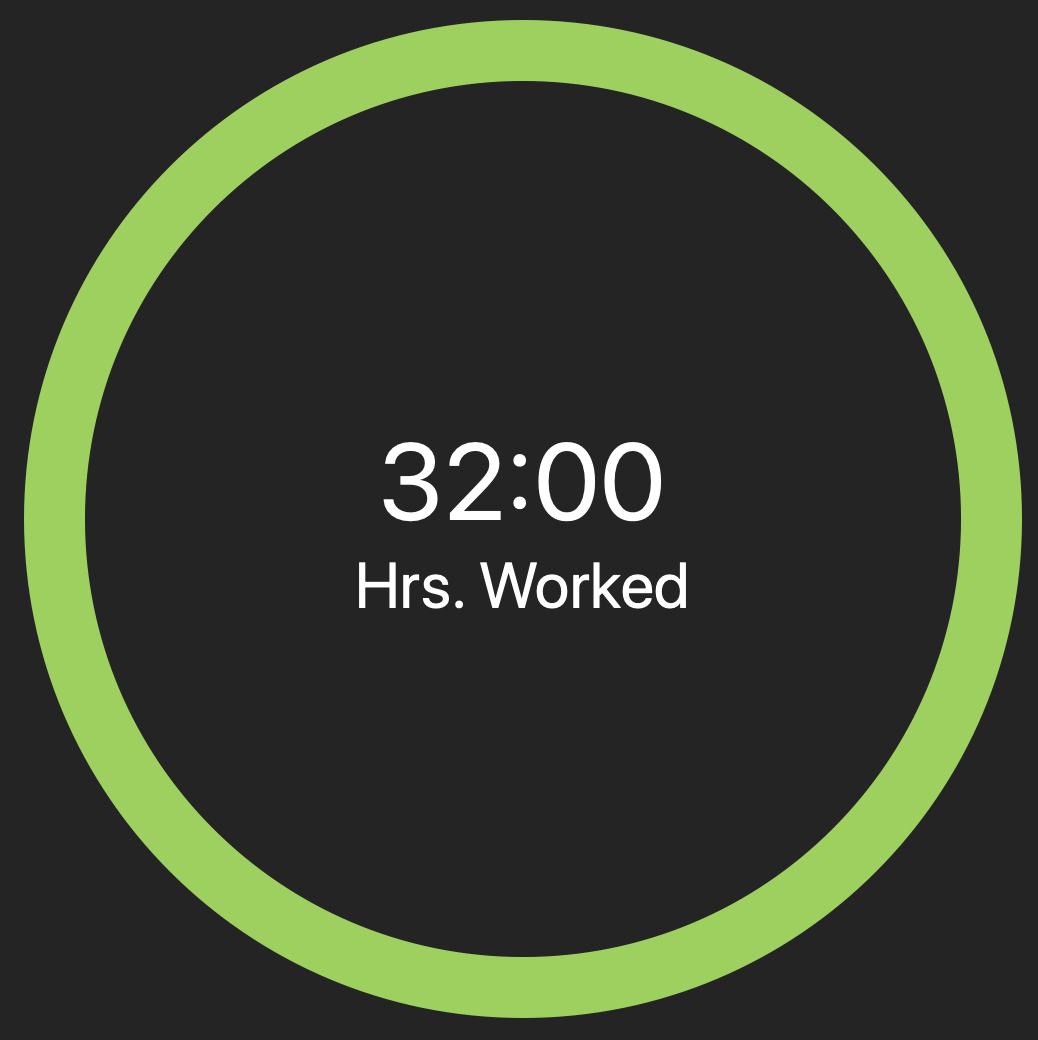
\includegraphics[width=0.5\linewidth]{TYME_TOT}
\end{center}
\end{figure}

\end{columns}
\end{frame}
% ---------------
\begin{frame}
\frametitle{Since last week}
\begin{columns}

\column{0.5\textwidth}
\begin{itemize}
\item Signal generator adds thermal and flicker noise.
\begin{itemize}
    \item Flicker noise function is not accurate yet.
\end{itemize}
\end{itemize}

\column{0.5\textwidth}
\begin{figure}[htbp]
\begin{center}
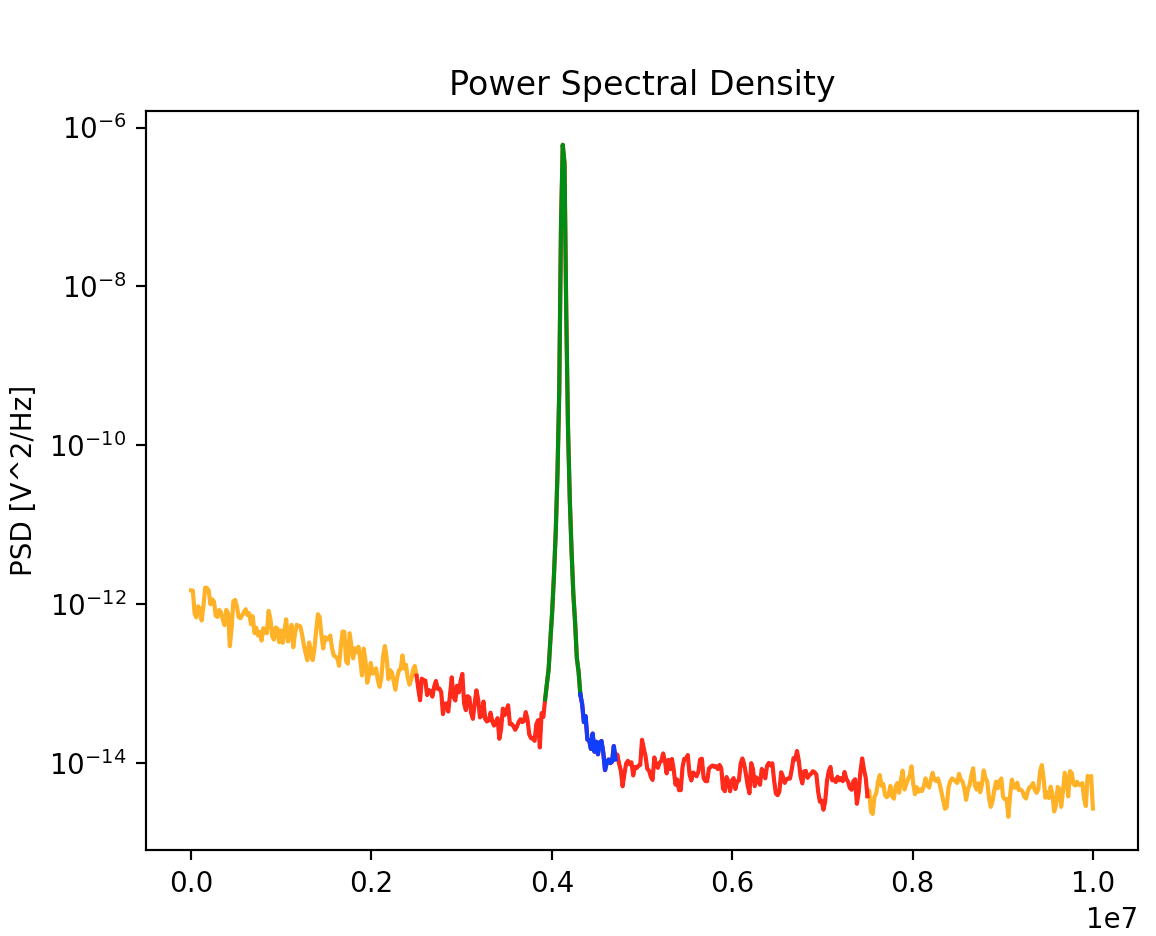
\includegraphics[width=\linewidth]{PSD}
\end{center}
\end{figure}

\end{columns}
\end{frame}

% ------------------- Timeline ---------------- %
\begin{frame}
\frametitle{Timeline}
\begin{figure}[htbp]
\begin{center}
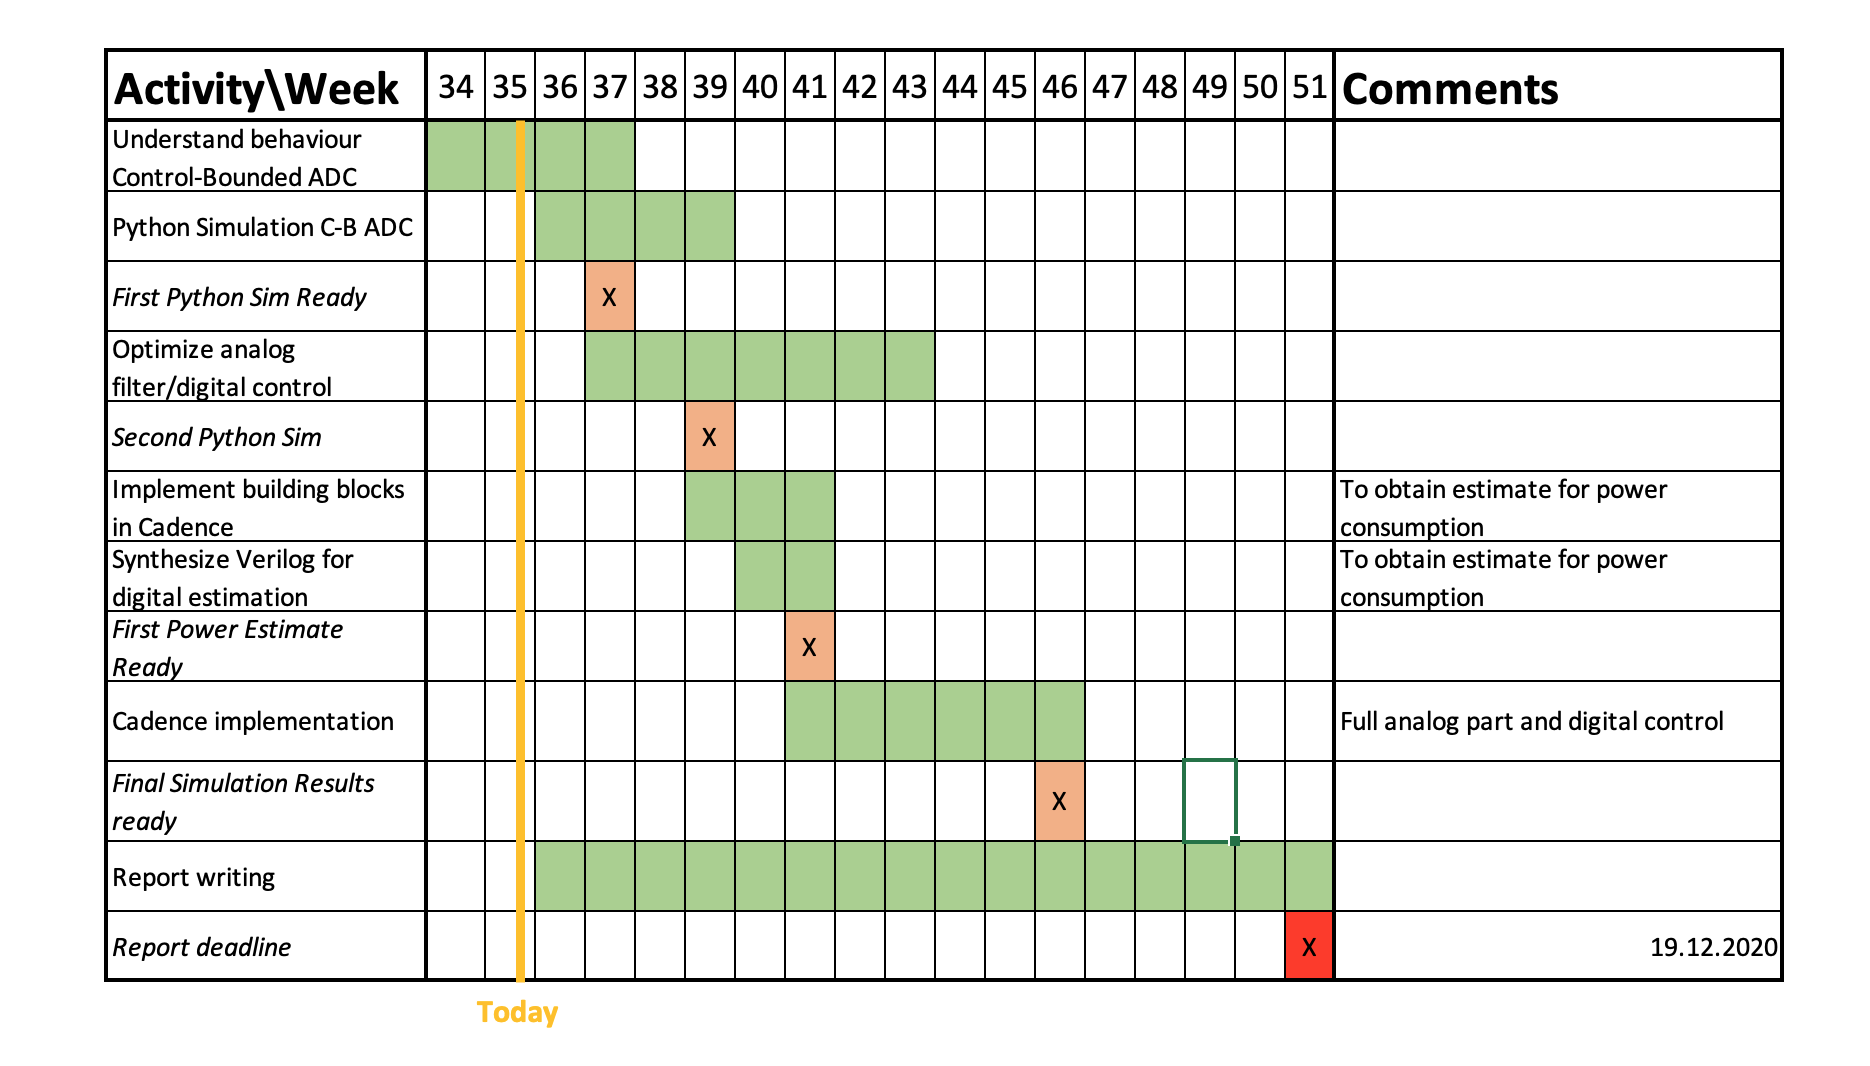
\includegraphics[width=\linewidth]{gantt}
\end{center}
\end{figure}
\end{frame}

% ------------------- Control Bounded ADC ---------------- %
\begin{frame}
\frametitle{Timeline}
\begin{figure}[htbp]
\begin{center}
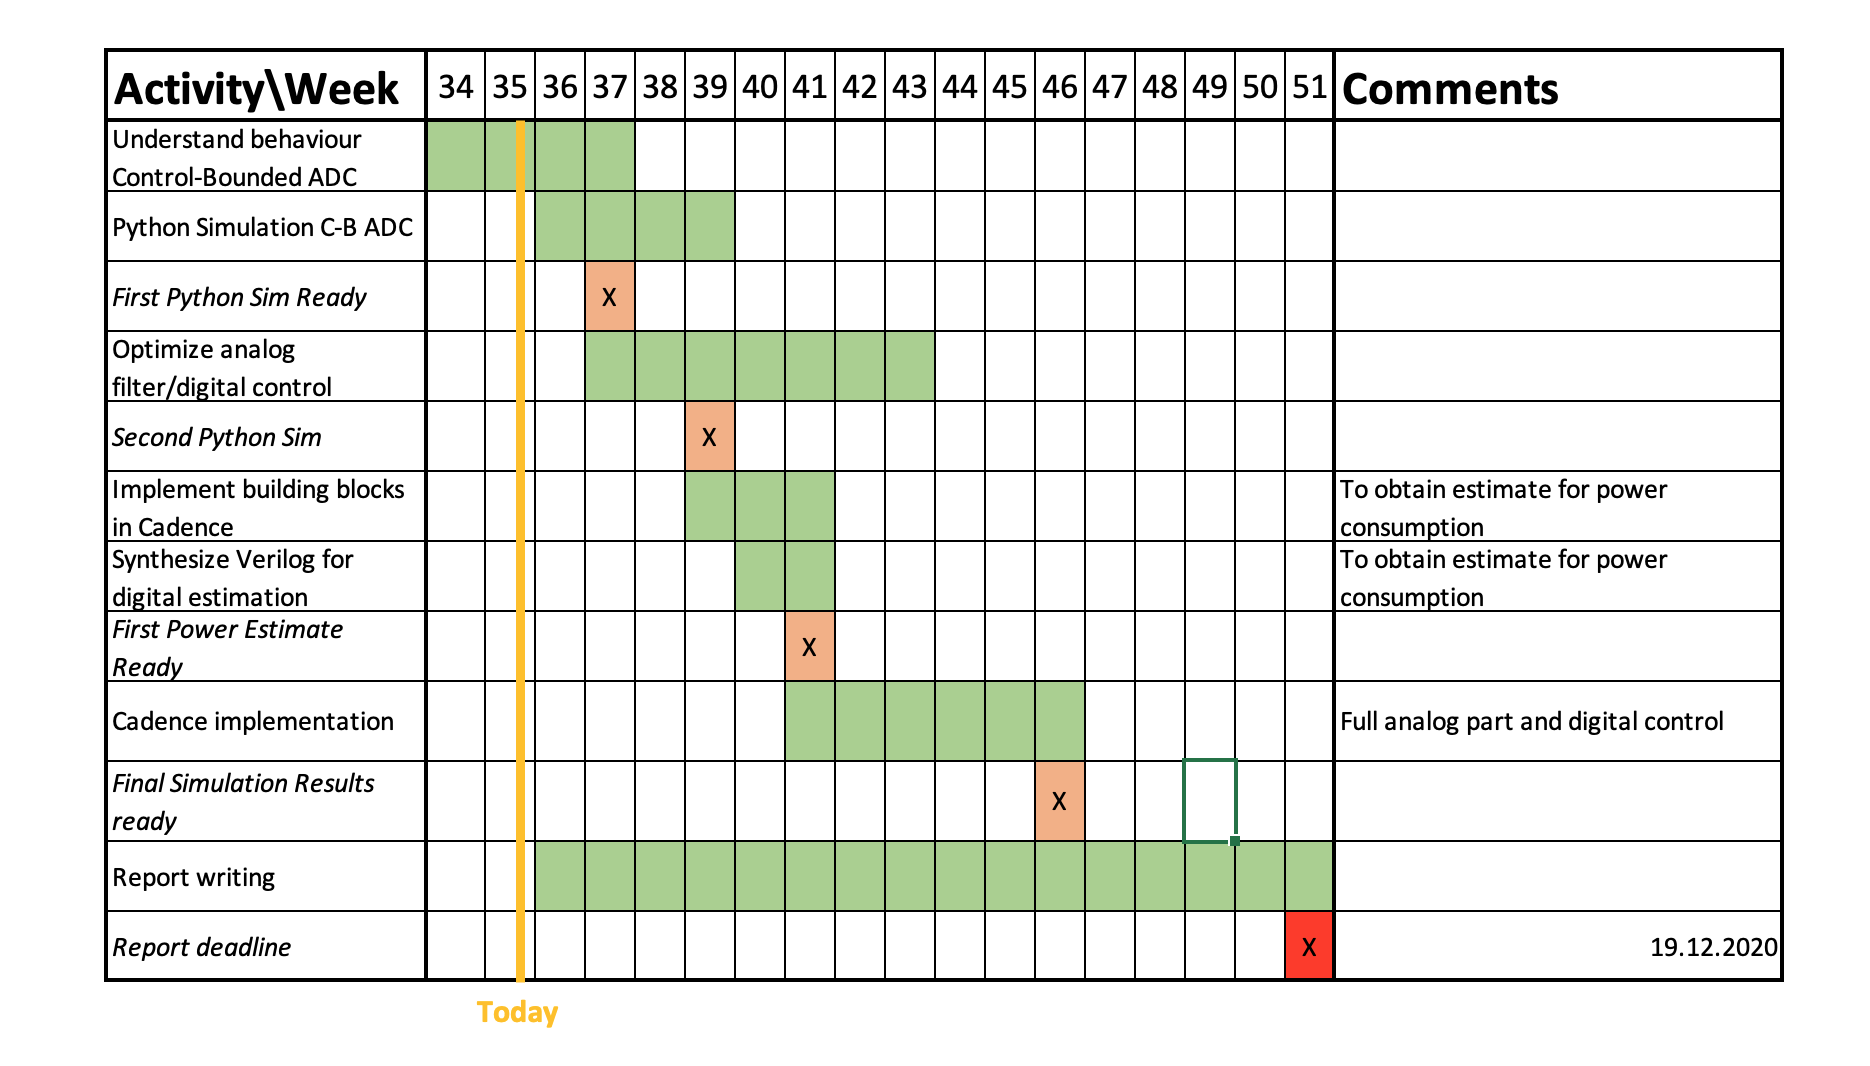
\includegraphics[width=\linewidth]{gantt}
\end{center}
\end{figure}
\end{frame}

% ------------------- Specs ---------------- %
\begin{frame}
\frametitle{Specs}
\begin{figure}[htbp]
\begin{center}
% !TEX root = update_0827.tex
% Table generated by Excel2LaTeX from sheet 'specs'
\begin{table}[htbp]
  \centering
  \caption{ADC Specs}
    \begin{tabular}{lccr}
    \rowcolor[rgb]{ 0,  0,  0} \textcolor[rgb]{ 1,  1,  1}{\textbf{Parameter}}	 & \textcolor[rgb]{ 1,  1,  1}{\textbf{Symbol}}
                             & \textcolor[rgb]{ 1,  1,  1}{\textbf{Value}}       & \textcolor[rgb]{ 1,  1,  1}{\textbf{Comment}}    \\
    Carrier Frequency & $f_c$ & \SI{5}{MHz} &                                                                                        \\
    Bandwidth & $\mathcal{B}$ & \SI{5}{MHz} & $2.5-7.5\si{MHz}$                                                                      \\
    Effective number of bits & ENOB & $>10$ bits &                                                                                    \\
    Noise density   & $\overline{V_n}$ & $<\SI[per-mode=symbol]{10}{\nano\voltnoise} $ & NF=$\SI{3}{dB}$                              \\
    Supply Voltage   & $V_{dd}$ & $<\SI{0.8}{V}$ &                                                                                    \\
    Power Consumption & $P_{tot}$ & $<\SI{50}{\micro W}$ & $\SI{500}{\atto J \per\text{c.s}}$\footnote{Walden FOM}\footnote{Hårete mål}
    \end{tabular}
  \label{tab:specs_data}
\end{table}



\end{center}
\end{figure}
\end{frame}



\end{document}
